Os três ``limites fundamentais'' são
\begin{itemize}
	\item $\displaystyle\lim_{x\to 0}\frac{\sin x}{x}=1$;
	\item $\displaystyle\lim_{x\to \pm\infty}\left(1+\frac{a}{x}\right)^x=e^a$;
	\item $\displaystyle\lim_{x\to 0}\frac{a^x-1}{x}=\ln(a)$.
\end{itemize}

\hrule

Vamos verificar de fato que estes limites são válidos.

\begin{itemize}
	\item Para o primeiro, devemos utilizar o Teorema do Confronto. Vamos tentar aproximar o valor de $\frac{\sin x}{x}$ utilizando funções trigonométricas.
	
	Para isso, devemos relembrar como ângulos em radianos são medidos, o que pode ser feito utilizando o círculo trigonométrico: Primeiro, consideramos um círculo de raio $1$ e um ângulo $x$ traçado sobre seu centro, conforme a figura abaixo:
	\[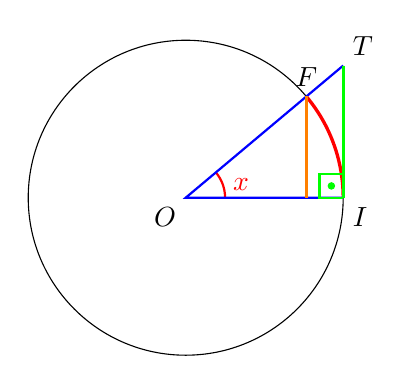
\begin{tikzpicture}[scale=2]
	    \node[below left] (O) at (0,0) {$O$};
	    \draw (0,0) circle (1);
	    \node[above] (F) at (40:1) {$F$}; 
	    \node[below right] (I) at (1,0) {$I$};
	    \node[above right] (T) at (1,0.839099631) {$T$};
	    \draw[very thick, red] (1,0) arc (0:40:1);
	    \draw[thick, red] (.25,0) arc (0:40:.25) node[midway,right] {$x$};
	    \draw[thick,blue] (1,0)--(0,0)-- (1,0.839099631);
	    \draw[very thick,green] (1,0.839099631)--(1,0);
	    \draw[thick,green] (1,0)--(1,.15)--(.85,.15)--(.85,0)--(1,0);
	    \draw[green,fill=green] (.925,.075) circle (0.02);
	    \draw[very thick,orange] (40:1)--(0.766044443118978,0);
	\end{tikzpicture}\]
	
	Nesta figura, temos que
	\begin{itemize}
	    \item O comprimento do segmento $\overline{OI}$ é igual a $1$.
	    \item A medida em radianos do ângulo $x$ coincide com o comprimento do arco em vermelho (entre os pontos $I$ e $F$).
	    \item O seno do ângulo $x$ é o comprimento do segmento em laranja.
	    \item A tangente do ângulo $x$ é o comprimento do segmento em verde.
	\end{itemize}
	
	Podemos agora verificar que $\sin(x)\leq x\leq \tan(x)$, analizando áreas de partes da figura acima:
	
	\begin{itemize}
	    \item O triângulo $\triangle IOF$ possui área dada pela metade do produto de sua base e sua altura, ou seja,
	    \[\operatorname{area}(\triangle IOF)=\frac{\sin x}{2}.\]
	    \[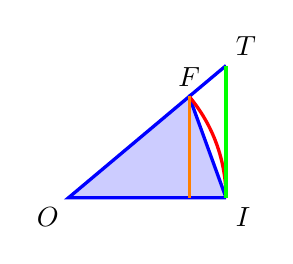
\begin{tikzpicture}[scale=2]
	    \node[below left] (O) at (0,0) {$O$};
	    \node[above] (F) at (40:1) {$F$}; 
	    \node[below right] (I) at (1,0) {$I$};
	    \node[above right] (T) at (1,0.839099631) {$T$};
	    \draw[very thick,blue,fill=blue!20] (1,0)--(0,0)-- +(40:1)--(1,0);
	    \draw[very thick,blue] (40:1) -- (1,0.839099631);
	    \draw[very thick, red] (1,0) arc (0:40:1);
	    
	    \draw[very thick,green] (1,0.839099631)--(1,0);
	    \draw[very thick,orange] (40:1)--(0.766044443118978,0);
	\end{tikzpicture}\]
	    \item A área total do círculo é igual a $2\pi$, e o setor $\angle IOF$ compreende uma fração de $\frac{x}{2\pi}$ de ``uma volta inteira'' pelo círculo. Portanto, este setor possui área
	    \[\operatorname{area}(\triangle IOF)=\frac{x}{2\pi}\cdot {\pi}=\frac{x}{2}.\]
	    \[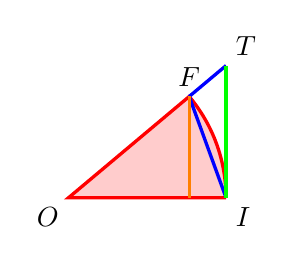
\begin{tikzpicture}[scale=2]
	    \node[below left] (O) at (0,0) {$O$};
	    \node[above] (F) at (40:1) {$F$}; 
	    \node[below right] (I) at (1,0) {$I$};
	    \node[above right] (T) at (1,0.839099631) {$T$};
	    \draw[very thick, red, fill=red!20] (1,0) arc (0:40:1) -- (0,0) -- (1,0);
	    \draw[very thick,blue] (40:1)--(1,0);
	    \draw[very thick,blue] (40:1) -- (1,0.839099631);
	    \draw[very thick,green] (1,0.839099631)--(1,0);
	    \draw[very thick,orange] (40:1)--(0.766044443118978,0);
	\end{tikzpicture}\]
	    \item O triâgulo $\triangle IOT$ possui área dada pela metade do produto de sua base e sua altura, ou seja,
	    \[\operatorname{area}(\triangle IOT)=\frac{\tan(x)}{2}.\]
	    \[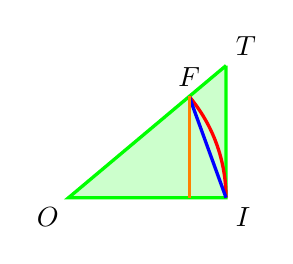
\begin{tikzpicture}[scale=2]
	    \node[below left] (O) at (0,0) {$O$};
	    \node[above] (F) at (40:1) {$F$}; 
	    \node[below right] (I) at (1,0) {$I$};
	    \node[above right] (T) at (1,0.839099631) {$T$};
	    \draw[very thick,green,fill=green!20] (1,0.839099631)--(1,0)--(0,0)--(1,0.839099631);
	    \draw[very thick, red] (1,0) arc (0:40:1);
	    \draw[very thick,blue] (40:1)--(1,0);
	    \draw[very thick,orange] (40:1)--(0.766044443118978,0);
	\end{tikzpicture}\]
	\end{itemize}
	
	Como $\triangle IOF\subseteq\angle IOF\subseteq\triangle IOT$ e a área de figuras menores é menor do que a área de figuras maiores, obtemos
	\[\frac{\sin(x)}{2}\leq\frac{x}{2}\leq\frac{\tan(x)}{2},\]
	ou seja,
	\[\sin(x)\leq x\leq\tan(x).\]
	
	Daí, obtemos que
	\[\frac{\sin(x)}{\tan(x)}\leq \frac{sin(x)}{x}\leq \frac{x}{x},\]
	ou seja,
	\[\cos(x)\leq \frac{\sin(x)}{x}\leq 1.\]
	Tomando $x\to 0$, temos que $\cos(x)\to 1$, e pelo \href{teo_do_confronto_moodle.html}{Teorema do Confronto} obtemos que $\frac{\sin(x)}{x}\to 1$. Isto mostra que
	\[\lim_{x\to 0}\frac{\sin(x)}{x}=1.\]
	
	\item Nós já sabemos que
	\[e=\lim_{y\to\infty}\left(1+\frac{1}{y}\right)^y\]
	(na verdade, esta é uma das definições que usamos). Vamos mostrar que o mesmo limite, porém no $-\infty$, também é válido.
	
	Por um lado, temos que
	\begin{align*}
	    e
	        &=\lim_{y\to\infty}\left(1+\frac{1}{y}\right)^y\\
	        &=\lim_{y\to\infty}\left(\frac{y+1}{y}\right)^y,\tag{E2.1}
	\end{align*}
	e por outro, que
	\begin{align*}
	    e
	        &=\lim_{y\to\infty}\left(1+\frac{1}{y}\right)^y\\
	        &=\lim_{z\to-\infty}\left(1-\frac{1}{z}\right)^{-z}\\
	        &=\lim_{z\to-\infty}\left(\frac{z-1}{z}\right)^{-z}\\
	        &=\lim_{z\to-\infty}\left(\frac{z}{z-1}\right)^z\tag{E2.2},
	\end{align*}
	onde realizamos a substituição $z=-y$ na segunda igualdade.	As expressões que aparecem em (E2.1) e em (E2.2) não são tão diferentes: são o quociente de dois monômios de grau $1$ elevado à variável dos monômios. Vamos tentar transformar uma destas expressões na outra. Para isso, vamos procurar uma nova variável $w$ de forma que
	\[\frac{w+1}{w}=\frac{z}{z-1}.\]
	A resolução desta equação nos dá $w=z+1$. Note que $w\to-\infty$ se, e somente se, $z\to-\infty$. Substituindo em (E2.2), obtemos
	\begin{align*}
	    e
	        &=\lim_{w\to-\infty}\left(\frac{w+1}{w}\right)^{w+1}\\
	        &=\lim_{w\to-\infty}\left(\frac{w+1}{w}\right)^w\cdot \left(\frac{w+1}{w}\right).\tag{E2.3}
	\end{align*}
	Estamos quase terminados, exceto que temos um fato ``$\frac{w+1}{w}$'' sobrando. Vamos aplicar a regra do produto para limites. Note que
	\begin{align*}
	    \lim_{w\to-\infty}\left(\frac{w+1}{w}\right)
	        &=\lim_{w\to-\infty}1+\frac{1}{w}\\
	        &=1
	\end{align*}
	e aplicando inversos, obtemos
	\begin{align*}
	    1
	        &=1^{-1}\\
	        &=\lim_{w\to-\infty}\left(\frac{w+1}{w}\right)^{-1}\tag{E2.4}.
	\end{align*}
	Assim, concluímos que
	\begin{align*}
	    e
	        &=e\cdot 1\\
	        &=\left(\lim_{w\to-\infty}\left(\frac{w+1}{w}\right)^w\cdot\left(\frac{w+1}{w}\right)\right)\cdot\left(\lim_{w\to-\infty}\left(\frac{w+1}{w}\right)^{-1}\right)\\
	        &\qquad\text{(por (E2.3) e (E2.4)}\\
	        &=\lim_{w\to-\infty}\left(\frac{w+1}{w}\right)^w\cdot\left(\frac{w+1}{w}\right)\cdot\left(\frac{w+1}{w}\right)^{-1}\\
	        &\qquad\text{(pela Regra do Produto)}\\
	        &=\lim_{w\to-\infty}\left(\frac{w+1}{w}\right)^w.\tag{E2.5}
	\end{align*}
	
	Juntando (E2.1) e (E2.5), concluímos que
	\[e=\lim_{y\to\pm\infty}\left(1+\frac{1}{y}\right)^{y}.\]
	
	Agora no caso geral, considere $a\in\mathbb{R}$. Se $a=0$, então claramente temos que
	\begin{align*}
	    \lim_{x\to\pm\infty}\left(1+\frac{0}{x}\right)^x
	        &=\lim_{x\to\pm\infty}1^x\\
	        &=1\\
	        &=e^0.
	\end{align*}
	
	Suponha então que $a\neq 0$. Vamos calcular
	\begin{align*}
	    \lim_{x\to\pm\infty}\left(1+\frac{a}{x}\right)^x
	        &=\lim_{x\to\pm\infty}\left(\left(1+\frac{1}{(x/a)}\right)^{x/a}\right)^a.
	\end{align*}
	Fazendo a substituição $y=x/a$, temos que $x\to\pm\infty$ se, e somente, $y\to\pm\infty$. Assim,
	\begin{align*}
	    \lim_{x\to\pm\infty}\left(1+\frac{a}{x}\right)^x
	        &=\lim_{y\to\pm\infty}\left(\left(1+\frac{1}{y}\right)^y\right)^a
	\end{align*}
	Como a função ``Potência em expoente $a$'' (que leva $x$ em $x^a$) é elementar, podemos passar o limite para dentro e obter
	\begin{align*}
	    \lim_{x\to\pm\infty}\left(1+\frac{a}{x}\right)^x
	        &=\left(\lim_{y\to\infty}\left(1+\frac{1}{y}\right)^y\right)^a\\
	        &=e^a.
	\end{align*}
	
	\item Vamos calcular $\lim_{x\to 0}\frac{a^x-1}{x}$. Seja $z=a^x-1$. Então $x=\log_a(z+1)$, e $x\to 0$ se, e somente se, $z\to 0$. Assim,
	\begin{align*}
	    \lim_{x\to 0}\frac{a^x-1}{x}
	        &=\lim_{z\to 0}\frac{z}{\log_a(z+1)}\\
	        &=\lim_{z\to 0}\frac{1}{((\log_a(z+1))/z)}\\
	        &=\lim_{z\to 0}\frac{1}{\log_a((z+1)^{1/z})}
	\end{align*}
	Lembre-se da regra de troca de bases para logaritmos: $\log_\alpha(\beta)=\frac{\log_c(\beta)}{\log_c(\alpha)}$. Logo,
	\begin{align*}
	    \lim_{x\to 0}\frac{a^x-1}{x}
	        &=\lim_{z\to 0}\ln(a)\frac{1}{\ln((z+1)^{1/z})}\\
	        &=\ln(a)\frac{1}{\left(\displaystyle\lim_{z\to 0}\ln((z+1)^{1/z})\right)}.
	\end{align*}
	
	Agora fazemos a substituição $t=\frac{1}{z}$. Temos que $z\to 0$ se, e somente se, $t\to\pm\infty$. Portanto,
	\begin{align*}
	    \lim_{x\to 0}\frac{a^x-1}{x}
	        &=\ln(a)\frac{1}{\left(\displaystyle\lim_{t\to\pm\infty}\ln\left(\left(\frac{1}{t}+1\right)^{t}\right)\right)}
	\end{align*}
	Como a função $\ln$ é elementar, podemos passar o limite para dentro e obter
	\begin{align*}
	    \lim_{x\to 0}\frac{a^x-1}{x}
	        &=\ln(a)\frac{1}{\displaystyle\ln\left(\lim_{t\to\pm\infty}\left(\frac{1}{t}+1\right)^{t}\right)}\\
	        &=\ln(a)\frac{1}{\ln(e)}\\
	        &=\ln(a).
	\end{align*}
\end{itemize}